\documentclass[journal]{IEEEtran}
\usepackage{graphicx,amsmath,array,url}
\graphicspath{{figures/}}
\begin{document}
\title{Software Verification of Wearable Safety Monitoring in NeuroGuardian X}
\author{[Author names in publication order]\thanks{[Department and institution, city, country]; [Corresponding author email]}}
\maketitle
\begin{abstract}Wearable safety software must preserve suspected emergencies while distinguishing missing measurements and unconfirmed notifications from valid evidence. We present a reproducible software-in-the-loop study of NeuroGuardian X, an ESP32-S3 and Flutter prototype with a personalized statistical profile and notification backend. The evaluation executes production decision code on 1,600 synthetic physiological cases, 3,600 motion-policy replays, five controller cases, and five isolated backend cases. An additional 5,400-case phase-grid experiment checks impact capture against an analytical sampling model. For random short impacts followed by immobility, increasing the original policy from 1 to 50 Hz raises capture from 14/200 to 199/200, but neither rate produces a critical flag because the settling transient cancels the countdown. Across the phase grid, capture rises from 44/900 at 1 Hz to 888/900 at 100 Hz, while every captured event is canceled. An exploratory recovery guard preserves escalation in 199/200 immobile-impact cases but also escalates 198/200 unworn-device impacts. The physiological engine assigns Normal to all 200 missing-input cases and rejects every stationary baseline history. These results establish reproducible counterexamples and isolate sampling, state persistence, evidence availability, and notification semantics as distinct verification targets. The study evaluates software behavior; it provides no patient-level diagnostic accuracy or end-to-end emergency-delivery evidence.\end{abstract}
\begin{IEEEkeywords}Wearable monitoring, software verification, fall alert, signal quality, sampling, state machines, reproducibility.\end{IEEEkeywords}
\section{Introduction}
A wearable safety system transforms measurements into a sequence of decisions: accept a signal, recognize an event, retain or cancel an alert, and communicate its status. A defect at any transition can invalidate the intended behavior even when individual sensor values appear plausible. Verification must therefore address both numerical outputs and the meaning of the states presented to the wearer or guardian. This study asks whether an implemented wearable prototype satisfies observable monitoring and escalation requirements before clinical or field evaluation.

NeuroGuardian X combines an ESP32-S3 sensor interface, a Bluetooth Low Energy (BLE) connection, a Flutter mobile application, and a Python notification backend. NeuroTwin is the project name for a personal statistical baseline and rule-based explanation engine. In this implementation it is not a mechanistic physiological model, a disease simulator, or a clinically validated digital twin. The current study evaluates software behavior before making claims about measurements obtained from a completed wrist-worn device.

We make three bounded contributions. First, we define an executable evaluation spanning the firmware motion function, the production mobile decision engine, and isolated notification contracts, with source hashes and trial-level outputs. Second, we separate impact capture from event persistence through a sampling-only ablation and a controlled phase-grid experiment with an analytical reference. Third, we connect the resulting counterexamples to explicit requirements for missing-data handling, recovery cancellation, and alert-status reporting. The contribution is a traceable verification case study, not a new clinically validated detector or a claim that simulation alone establishes user safety.

The measured system is software-in-the-loop. Electronics, battery life, skin contact, radio timing, Android background execution, internet transport, and guardian response are outside its scope. Scenario names describe constructed inputs; no participants, patient recordings, or live emergency messages were involved.

\section{Related Work And Evaluation Scope}
SisFall provides recorded falls and activities of daily living acquired at 200 Hz [1]. Such recordings support activity-dependent evaluation, but a high-rate dataset does not by itself test how a particular implementation samples, retains, or cancels an event. Our generated impulses isolate these software mechanisms. They are not derived from SisFall, and the percentages reported here are not comparable with classification metrics measured on its recordings.

Bagala et al. evaluated 13 accelerometer-based algorithms on 29 real-world falls and reported substantial differences from results obtained with simulated falls [2]. Their study examines external performance; ours asks an earlier question about correctness under controlled inputs. The two forms of evidence are complementary. A software counterexample can expose an implementation problem without estimating its prevalence among real users.

Hongn et al. describe wearable physiological recordings collected during acute stress and structured exercise [3]. These recordings address activity context and physiological measurement, whereas our stress and exercise scenarios vary scalar software inputs. The distinction matters: increased heart rate or electrodermal values can probe score behavior without supplying a clinical stress label. We do not estimate stress-detection accuracy.

MIT-BIH contains 48 half-hour two-channel ECG records sampled at 360 Hz [4], [5], while this prototype transmits a periodic ECG scalar. Scalar-amplitude deviation cannot be equated with rhythm classification. Exam-stress [6], Sudden Cardiac Death Holter [7], and induced-stress/exercise [8] recordings are additional future resources, not study inputs. None of these records was used for fitting or testing; training-data use is zero.

Metamorphic testing evaluates relations between executions when a complete output oracle is difficult to obtain [9]. This motivates controlled transformations such as replacing available measurements with missing ones, changing activity context, or increasing temporal resolution while retaining the policy. We use such comparisons to interpret behavior, alongside a direct numerical oracle for the phase-grid control. This is not a claim to introduce a new metamorphic-testing method or to provide a complete formal verification of the application.

The research questions are: RQ1, does the personal-profile engine distinguish missing or low-quality evidence from an ordinary supported result; RQ2, how do sampling rate and cancellation policy separately affect capture and escalation; and RQ3, which controller and notification states are actually supported by recorded evidence? All comparisons are internal to the evaluated prototype. We do not benchmark commercial watches or claim that the failure modes are unique to this device.

\section{System Architecture And Implementation}
\begin{figure}[!t]\centering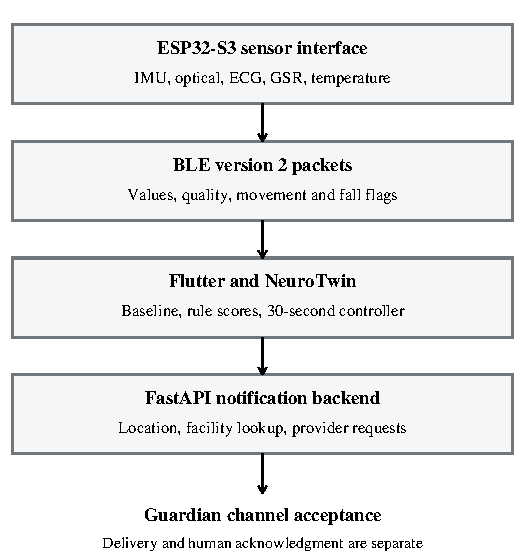
\includegraphics[width=\columnwidth]{architecture.pdf}\caption{Prototype data path. Software boundaries are exercised independently. Arrows do not imply that the complete hardware-to-guardian path was tested.}\end{figure}
\subsection{Wearable and packet interface}
The inspected firmware uses Arduino C++ on an ESP32-S3. It contains an MPU6050 motion path, analog GSR and ECG inputs, a battery input, an SOS button, and buzzer/vibration control. Optional compile-time paths exist for a MAX30102 optical module and a TinyGPSPlus GNSS receiver; both are disabled in the inspected configuration. Pressure and altitude are placeholders, and a dedicated calibrated temperature measurement path is unfinished. The MAX30102 internal temperature path, when enabled, should not be interpreted as an independently validated body-temperature measurement.

Version 2 packets carry JSON fields for time, heart rate, oxygen saturation, HRV, GSR, temperature, ECG scalar, motion axes, quality, position, battery, and event flags. BLE requests a 517-byte maximum transmission unit; negotiation and delivery are not measured. Motion acquisition and buildMotionState execute inside notifyMetrics at a nominal one-second interval only while deviceConnected is true. State advancement is consequently tied to the connected notification loop, excluding scheduling jitter and missed intervals from the idealized replay.

\subsection{Mobile application and NeuroTwin}
The Flutter application parses the packet into a Metrics object. NeuroTwin combines a signal-quality view, an activity-dependent personal baseline, trend summaries, and weighted rule scores. The baseline uses at most 120 eligible preceding samples. An overall profile is marked ready at 20 eligible samples; individual metric readiness uses 12 samples. These sample-count checks are software conventions and do not establish that a stable multi-day physiological baseline has been learned.

For metric x with n eligible samples, the baseline mean, sample standard deviation, and current normalized deviation are computed as follows. A metric-specific floor prevents division by a very small standard deviation.

\begin{equation}\begin{aligned}\mu&=\frac{1}{n}\sum_{i=1}^{n}x_i,\\s&=\sqrt{\frac{\sum_{i=1}^{n}(x_i-\mu)^2}{n-1}}.\end{aligned}\end{equation}
\begin{equation}z=\frac{x_{\mathrm{current}}-\mu}{\max(s,s_{\min})}.\end{equation}
Standard-deviation floors are 3 beats/min for heart rate, 0.8 percentage points for oxygen saturation, 5 ms for HRV, 4 arbitrary units for GSR, 0.2 degrees C for temperature, and 0.08 mV for ECG. Eligibility requires acceptable contact, quality at least 0.45, compatible activity, and usable physiology. It also rejects all samples with movementDetected false; the stationary-history experiment evaluates that condition.

Quality values are provided by the firmware or estimated from value availability and motion. NeuroTwin averages PPG, ECG, GSR, temperature, and motion quality and declares the result reliable when the average is at least 0.55 and watch fit is acceptable. These quality numbers are heuristics, not empirically calibrated probabilities. GPS readiness is handled separately. A high aggregate quality does not validate every individual channel.

\subsection{Composite score and labels}
Let S denote the stress score, C the existing cardiac-related rule score, E the ECG-scalar anomaly score, F the motion/fall score, O the oxygen-related load, and T the temperature-related load, each on a 0-100 scale. The current composite is:

\begin{equation}R_0=0.18S+0.22C+0.18E+0.26F+0.10O+0.06T.\end{equation}
For unreliable quality without a fall, the score is multiplied by 0.72. A fall with no movement sets a minimum score of 82, and the Critical fall activity sets a minimum of 92. A non-fall case without a ready baseline is capped at 72. Labels change at scores of 30, 60, and 80: Normal, Observe, Warning, and Critical Review. Although the application uses probability terminology for some components, this paper calls them scores because no probability calibration has been performed.

Stress combines GSR, HRV, heart-rate and temperature deviations with recent transmitted stress values and activity context. The ECG component uses scalar amplitude, baseline deviation, and HRV load. Implemented trend windows span five minutes, thirty minutes, and one hour; the experimental histories do not validate those durations.

\subsection{Alert controller and backend}
A fall signal starts the mobile 30-second countdown; a subsequent non-fall movement packet cancels it. Immediate escalation uses a heart-rate drop of at least 20 beats/min, compared with 22 in firmware, or Critical fall activity. Timing uses DateTime.now and periodic callbacks, so tests use real elapsed time rather than assuming the test framework virtualizes that clock.

The backend accepts an alert containing event information, coordinates, guardian settings, and optional medical facilities. If the list is absent, it can query Google Places Nearby Search [10]. Facility discovery returns information about places; it is not a hospital dispatch agreement. WhatsApp and push are separate provider paths. The current response includes success and delivery fields based on provider-call outcomes, while the webhook handler acknowledges receipt without retaining a message-delivery history. The controlled backend tests examine this contract, not a live service.

\section{Experimental Methods}
\subsection{Provenance and execution boundaries}
Experiments ran on Windows on 17 September 2026 against app version 0.4.0+4, Flutter 3.19.5, and Dart 3.3.3. Backend versions were Python 3.10.10, FastAPI 0.141.1, and HTTPX 0.28.1; native compilation used Microsoft C++ version family 14.50. Production sources were not modified. SHA-256 hashes identify the evaluated working tree, including changes beyond its base Git commit.

The host harness extracts buildMotionState, MotionSample, and relevant constants verbatim. It substitutes a controllable millisecond clock, released SOS button, and inert outputs. The decision function runs as native C++ with single-precision motion values, not as ESP32 processor or radio emulation. Connected operation is assumed.

Flutter tests import the production Dart classes. Backend tests import endpoint functions with dotenv disabled, provider configuration removed, and notification/facility providers replaced by stubs. Network-client construction is blocked to prevent synthetic alerts reaching real contacts.

\subsection{Evaluation requirements}
The test oracles are operational requirements rather than clinical diagnoses. R1 requires absent current physiology to remain distinguishable from an ordinary supported result. R2 requires otherwise eligible stationary rest to contribute to a resting profile. R3 requires a captured impact followed by continued immobility to retain the countdown until escalation. R4 requires explicit recovery or user cancellation to stop an active countdown. R5 requires an immediate-trigger reason to identify evidence actually present. R6 requires provider acceptance to remain distinct from delivery and acknowledgment. These requirements express the intended prototype behavior and the claims its interface can support; they are not a certification standard.

\subsection{NeuroTwin synthetic cases}
Seeds 17, 29, 43, 71, and 101 each generate 40 repetitions per scenario: 200 cases per scenario and 1,600 evaluations. Each case has 120 preceding one-second observations and one current observation, excluded from its baseline. Histories use ordinary resting inputs with movementDetected true except in the stationary scenario, permitting comparison with otherwise eligible quiet-rest histories.

\begin{table}[!t]\caption{CURRENT SYNTHETIC INPUT RANGES}\centering\scriptsize\setlength{\tabcolsep}{2pt}
\begin{tabular}{p{0.260\columnwidth}p{0.650\columnwidth}}\hline
Scenario & Changed inputs\\\hline
Normal & HR 68-76; SpO2 97-99; HRV 45-55; GSR 28-36\\
Stationary & Same ranges; all movement flags false\\
Stress shift & HR 95-115; HRV 15-25; GSR 75-90; stress 75-90\\
Exercise & HR 120-145; HRV 20-35; activity Running\\
ECG scalar shift & ECG 1.6-2.0 mV; other values ordinary\\
Poor contact & Quality 0.05-0.20; fit false; shifted numeric values\\
Missing & HR and temperature zero; optional vitals absent\\
Fall inactive & Fall flag true; movement false; ordinary vitals\\
\hline\end{tabular}\end{table}
Ordinary continuous ranges are temperature 36.5-36.8 degrees C, ECG 0.55-0.69 mV, transmitted stress 25-35, and quality 0.85-0.95. Integer endpoints are inclusive; continuous upper endpoints are excluded. GSR is an arbitrary 0-100 scalar, and HRV is supplied rather than waveform-derived. These are engineering inputs, not clinical reference intervals.

The poor-contact case retains shifted numeric values while lowering supplied quality and contact status, separating channel presence from channel trust. The missing case removes physiological measurements but preserves motion input. The ECG-scalar case is a feature perturbation, not an arrhythmia label. Each evaluation records component scores, the composite category, quality reliability, baseline eligibility, explanations, and input values. Means and sample standard deviations describe algorithm outputs; no generated scenario is treated as disease ground truth.

\subsection{Motion generator and sampling comparison}
The motion experiment uses the same five seeds and 40 repetitions per seed for each of six trace families: quiet, walking, impact followed by immobility, impact followed by recovery, impact with a heart-rate step, and an unworn-device impact. There are 1,200 parameterized traces. Each lasts 45 seconds and is independently replayed at 1 Hz and 50 Hz. For an impact trace, peak time t0 is uniform on [5,6) seconds, width w is uniform on [0.08,0.24) seconds, and peak magnitude A is uniform on [2.8,4.2) g. A low-amplitude sinusoid is added to the 1 g baseline.

\begin{equation}\begin{aligned}a(t)&=1+0.004\sin(2\pi\,0.7t+\phi)\\&\quad+(A-1)\max\!\left(0,1-\frac{2|t-t_0|}{w}\right).\end{aligned}\end{equation}
The phase phi is uniform on [0,2 pi). Quiet and walking traces omit the impact term. Walking adds a 0.35 g sinusoid at 1.8 Hz; recovery adds the same oscillation eight seconds after the peak. The heart-rate-step trace changes from 75 to 45 beats/min at the start of the impact support. The unworn-device trace intentionally uses the same scalar motion family as the immobile-impact trace, because a magnitude signal alone does not encode whether the device is attached to a person. The generator does not model orientation, skin contact, sensor saturation, or a population distribution of real falls.

The production policy starts a countdown when magnitude exceeds 2.6 g. It defines movement as the absolute difference between successive magnitudes exceeding 0.10 g. If the timer is active and movement is detected without a concurrent impact, it cancels the timer. A critical flag follows 30 seconds without cancellation or a qualifying concurrent heart-rate drop. Replay uses the same continuous trace parameters for all policies; it does not optimize separate inputs to favor an alternative.

\begin{figure}[!t]\centering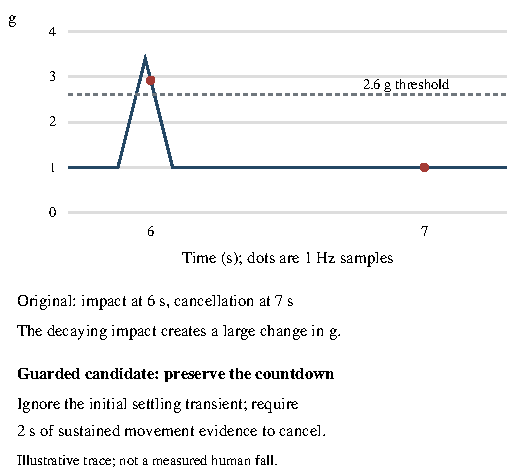
\includegraphics[width=\columnwidth]{sampling_failure.pdf}\caption{Illustrative synthetic counterexample. A sample on the impulse starts the timer, but the next sample near 1 g produces a large magnitude difference and cancels it.}\end{figure}
\subsection{Experimental guarded recovery policy}
A separate Python policy is evaluated only as an exploratory diagnostic alternative. It samples at 50 Hz, latches the same 2.6 g impact, and retains the same 30-second timeout. It ignores recovery cancellation for the first 1.5 seconds. Thereafter, movement evidence is a peak-to-peak magnitude range greater than 0.18 g over the previous 0.5 seconds. Cancellation requires that evidence to persist for two seconds. The candidate retains an adjacent-sample heart-rate-drop check, allowing its timing weakness to remain visible. It is not installed in the app or firmware.

Guard parameters were engineering choices made during debugging, without patient training or held-out selection. Original-policy replay at 50 Hz isolates sampling from cancellation changes. Python and C++ policies are compared by state transitions, not execution speed.

\subsection{Endpoints and controller contracts}
For each policy and trace, the harness records whether a fall/countdown flag appears, whether cancellation occurs, and the first critical-flag time. The randomized motion experiment contains 3,600 policy-trace evaluations, with 200 traces per family and policy. Capture is a threshold/state event; escalation is a later critical flag, not an outgoing message. Wilson 95\% intervals summarize binomial proportions under the specified generator [11]. Policies share trace parameters, so their observations are paired rather than independent groups. No clinical power analysis or null-hypothesis significance claim is made. The deterministic phase-grid experiment below is reported separately without binomial confidence intervals.

Five controller cases cover fall-then-silence, movement after five seconds, manual reset, stillness without fall, and Critical fall activity. No-response cases run concurrently for 32 seconds; the timeout is one observation, not a latency distribution. Backend cases enumerate all four provider outcomes and one failed-delivery webhook. No physical disconnection, Android suspension, or live provider is tested.

\subsection{Analytical sampling control}
A separate deterministic experiment removes the low-amplitude sinusoid from (4), producing one triangular impulse on a constant 1 g baseline. With threshold theta = 2.6 g, peak A > theta, and support width w, the time spent above threshold is d = w(A - theta)/(A - 1). If the sample phase is uniform over a period 1/f, the probability that at least one sample intersects this interval is:

\begin{equation}d=w\frac{A-\theta}{A-1}\end{equation}
\begin{equation}P_{\mathrm{capture}}(f)=\min(1,fd)\end{equation}
Equation (6) follows because phases producing capture occupy length d within a sampling period when d < 1/f; otherwise every phase intersects the above-threshold interval. Equality at a threshold has zero probability under continuous phase. This is a sampling result for the constructed impulse, not a model of human falls. It predicts capture only, making no assumption that the implemented timer survives afterward.

We execute the extracted original function at f in {1, 5, 10, 25, 50, 100} Hz, w in {0.08, 0.16, 0.24} s, and A in {2.8, 3.5, 4.2} g. Each combination uses 100 midpoint phases, u\_j = (j + 0.5)/100 for j = 0,...,99, with peak time 5 + u\_j/f seconds. Each trace lasts 38 seconds and supplies constant heart rate 75 beats/min and connected status. The design yields 900 traces per rate and 5,400 native executions. The discrete oracle checks whether any sampled magnitude exceeds theta; the continuous-phase reference averages (6) across the nine peak/width combinations. The grid is a follow-up diagnostic extension, not a random sample, held-out evaluation, or external test set.

\section{Results}
\subsection{NeuroTwin score and baseline behavior}
\begin{table}[!t]\caption{PRODUCTION ENGINE OUTPUTS FOR 200 CASES PER ROW}\centering\scriptsize\setlength{\tabcolsep}{2pt}
\begin{tabular}{p{0.286\columnwidth}p{0.307\columnwidth}p{0.317\columnwidth}}\hline
Scenario & Risk mean (SD) & Ready / usable\\\hline
Normal & 6.15 (0.53) & 200 / 200\\
Stationary & 16.03 (0.53) & 0 / 200\\
Stress shift & 23.69 (1.29) & 200 / 200\\
Exercise & 19.80 (1.19) & 0 / 200\\
ECG scalar & 16.82 (0.77) & 200 / 200\\
Poor contact & 22.07 (1.08) & 200 / 0\\
Missing & 0.95 (0.04) & 200 / 0\\
Fall inactive & 82.00 (0.00) & 0 / 200\\
\hline\end{tabular}\end{table}
In Table II, Ready is the number of ready baseline profiles and usable is the number passing the current aggregate-quality rule. All normal histories become ready, whereas no stationary history does. All exercise cases also have an unready baseline because their preceding history is resting and the current context is running. This latter result is expected for a new activity context; the stationary exclusion is more consequential because quiet rest is a legitimate monitoring state. All counts refer to the program rules, not a validated quality reference.

\begin{figure}[!t]\centering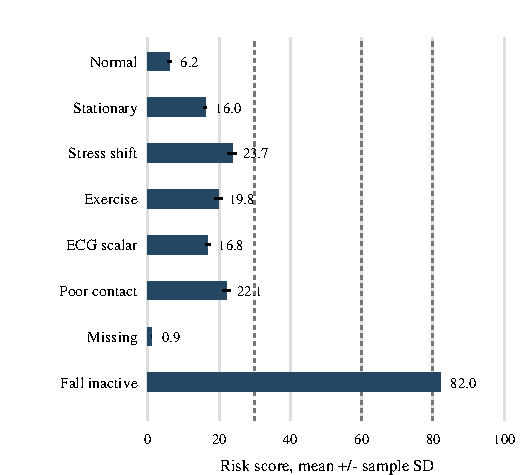
\includegraphics[width=\columnwidth]{risk_results.pdf}\caption{Production NeuroTwin risk means with sample-standard-deviation error bars. Dashed lines mark category thresholds at 30, 60, and 80; none is a medically calibrated threshold.}\end{figure}
Normal and stationary cases have mean scores of 6.15 and 16.03, respectively. The 9.88-point difference follows the stillness contribution to the motion/fall score, although the scenario contains no fall. The stress-shift component rises to 64.29 on average, but the composite remains 23.69. Similarly, the ECG-scalar component averages 69.88, while its composite averages 16.82. All 200 cases in each of these groups retain the Normal category. This is a score-aggregation observation, not evidence that the corresponding synthetic shifts are medically harmless.

All 200 poor-contact inputs are marked unreliable, and their ECG component is zero, yet their stress component remains elevated at a mean of 78.26. This occurs because the separate stress-pattern path still consumes numeric values and recent stress history. Reducing the final score is not equivalent to removing untrusted contributions from every explanation. The 200 missing-signal cases all receive the Normal category despite zero usable physiological channels. Their ready profile reflects the preceding good history, not valid current measurements. The appropriate operational interpretation is unavailable current evidence; a categorical Normal display can conceal that distinction.

Every fall-inactive input reaches exactly 82 and Critical Review because the explicit minimum dominates the weighted score. This consistency confirms execution of the override. It does not establish that a true fall has been detected, since the experiment supplies the fall flag directly. No disease-classification accuracy, sensitivity, specificity, or receiver-operating-characteristic area is calculated.

\subsection{Impact capture and critical flags}
\begin{table}[!t]\caption{CAPTURE / CRITICAL COUNTS OUT OF 200}\centering\scriptsize\setlength{\tabcolsep}{2pt}
\begin{tabular}{p{0.294\columnwidth}p{0.205\columnwidth}p{0.205\columnwidth}p{0.205\columnwidth}}\hline
Trace family & Orig. 1 Hz & Orig. 50 Hz & Guard 50 Hz\\\hline
Quiet & 0 / 0 & 0 / 0 & 0 / 0\\
Walking & 0 / 0 & 0 / 0 & 0 / 0\\
Impact immobile & 14 / 0 & 199 / 0 & 199 / 199\\
Impact recovery & 10 / 0 & 198 / 0 & 198 / 0\\
Impact HR drop & 9 / 9 & 199 / 0 & 199 / 199\\
Unworn impact & 8 / 0 & 198 / 0 & 198 / 198\\
\hline\end{tabular}\end{table}
At 1 Hz, the original function captures 14 of 200 immobile-impact traces (7.0\%) and generates zero critical flags. At 50 Hz it captures 199 (99.5\%) but still generates zero critical flags. The reason is the cancellation branch: as the impulse decays toward 1 g, the inter-sample difference exceeds 0.10 g while the magnitude is below 2.6 g. The timer is therefore canceled by the settling transient. Increased sampling alone does not repair this state-transition rule.

\begin{figure}[!t]\centering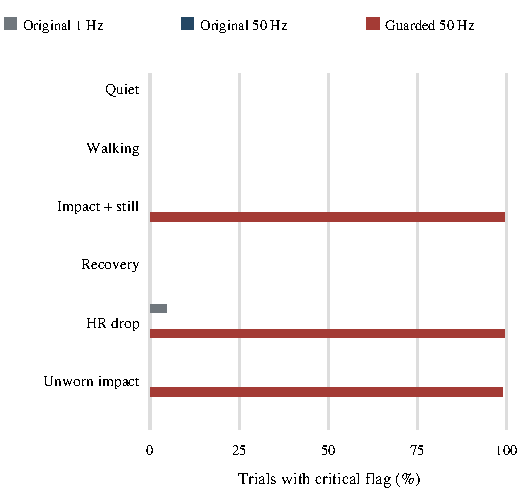
\includegraphics[width=\columnwidth]{motion_results.pdf}\caption{Critical-flag rate for each synthetic family and policy. The unworn-impact result is an adverse false-escalation case, not a successful detection.}\end{figure}
The guarded candidate escalates 199/200 immobile-impact traces (99.5\%; Wilson 95\% interval 97.22-99.91\%) and 0/200 recovery traces (upper Wilson bound 1.88\%). It also escalates 198/200 unworn-device impacts (99.0\%; interval 96.43-99.73\%). Across the five seeds, immobile-impact escalation ranges from 39/40 to 40/40; recovery remains 0/40, and unworn-impact escalation ranges from 39/40 to 40/40. Thus, the behavior is not confined to one seed. The adverse unworn result prevents interpreting the retained countdown as reliable discrimination of a human emergency.

For the heart-rate-step family, the original 1 Hz policy produces nine immediate critical flags. The original 50 Hz policy produces none, although it captures 199 impacts. At the higher rate, the heart-rate step can be observed before magnitude crosses the impact threshold; by the time the countdown starts, the adjacent-sample heart-rate difference is zero. The guarded candidate eventually escalates 199 cases after its countdown, rather than restoring immediate escalation. This result exposes an event-association problem: faster acquisition can reveal timing assumptions that are hidden by coarse sampling. A recent-event buffer would be a separate design change requiring its own evaluation.

\subsection{Sampling control and persistence}
\begin{table}[!t]\caption{DETERMINISTIC SAMPLING CONTROL}\centering\scriptsize\setlength{\tabcolsep}{2pt}
\begin{tabular}{p{0.151\columnwidth}p{0.273\columnwidth}p{0.239\columnwidth}p{0.242\columnwidth}}\hline
Rate Hz & Capture / 900 & Model \% & Critical\\\hline
1 & 44 & 5.18 & 0\\
5 & 232 & 25.90 & 0\\
10 & 444 & 49.57 & 0\\
25 & 704 & 78.37 & 0\\
50 & 832 & 92.59 & 0\\
100 & 888 & 98.77 & 0\\
\hline\end{tabular}\end{table}
Table IV reports the phase-grid results. Capture increases from 44/900 (4.89\%) at 1 Hz to 888/900 (98.67\%) at 100 Hz. All 5,400 outputs agree with the discrete capture oracle. Across the 54 rate/width/peak cells, the maximum absolute difference between the 100-phase capture fraction and (6) is 0.889 percentage points, consistent with the finite grid. Every captured event is subsequently canceled, and no critical flag appears. Agreement at the capture stage therefore coexists with a persistence failure.

The grid and randomized families use different peak/width weightings and baseline signals. In particular, 832/900 captures at 50 Hz in the grid must not be pooled with 199/200 in the randomized immobile-impact family or interpreted as a replication discrepancy. Both experiments isolate the same distinction: increased temporal resolution can improve threshold observation while leaving the cancellation branch unchanged. The 100 Hz result is specific to the tested widths and amplitudes; it is not evidence that no higher rate or different waveform could change the state behavior.

\subsection{Controller and backend observations}
The production mobile controller triggers after 30.012 seconds in the single fall-then-silence run. Movement at five seconds cancels the countdown, manual reset returns it to Idle, and stationary input without a fall remains Idle. A Critical fall activity triggers immediately and is labeled with the sudden-heart-rate-drop reason even though that case supplies no preceding heart-rate decline. Thus, both stale-input handling and trigger-reason provenance require attention. Continued packet silence is currently treated as no-response continuity, rather than distinguished from sensor disconnection.

The backend returns success when either provider stub accepts, and false when both reject. Three synthetic medical facilities appear in each response. This confirms the programmed Boolean aggregation and facility-list path. The failed-delivery webhook is acknowledged with an ok/received response, but the handler maintains no delivery record or alert-state transition. Provider acceptance, handset delivery, and human acknowledgment are therefore separate claims; only the first is represented by these tested return values.

\subsection{Requirement-level assessment}
\begin{table}[!t]\caption{REQUIREMENTS AND OBSERVED COUNTEREXAMPLES}\centering\scriptsize\setlength{\tabcolsep}{2pt}
\begin{tabular}{p{0.221\columnwidth}p{0.463\columnwidth}p{0.221\columnwidth}}\hline
Requirement & Evidence & Result\\\hline
R1 Availability & 200/200 missing cases Normal & Violated\\
R2 Rest profile & 0/200 stationary histories ready & Violated\\
R3 Persistence & 3144/3144 captured events canceled & Violated\\
R4 Cancellation & Movement and reset cases cancel & Observed\\
R5 Provenance & HR-drop reason without decline & Violated\\
R6 Alert status & No retained delivery transition & Incomplete\\
\hline\end{tabular}\end{table}
Table V maps evidence to the declared requirements. Observed means that the specific local case satisfied the intended transition, not that all executions satisfy it. A finite test can establish a counterexample to a requirement but cannot establish universal safety. The matrix also distinguishes missing functionality, such as delivery-state persistence, from a numerical false classification.

\section{Discussion And Design Implications}
The central finding is a separation between observing an input, retaining an event, and establishing an outcome. Sampling determines whether an impulse crosses the threshold in a sampled sequence. Cancellation logic determines whether that event survives until timeout. Channel validity determines whether a physiological score has interpretable evidence. Provider-return values determine whether an alert request was accepted, not whether a guardian received or acted on it. A single aggregate accuracy or success label would conflate these independently testable properties.

Motion acquisition should be separated from the connected BLE notification loop, with a bounded event record retained across communication interruptions. The guarded-policy ablation shows that windowed recovery evidence can preserve a countdown that the original difference rule cancels. Its false escalations also show why recovery hysteresis alone is insufficient. Contact and wearer-state evidence need their own measurement and validation path; neither a transient acceleration change nor prolonged stillness establishes that a person has recovered or become unconscious.

The unworn family exposes a separate observability limit. If a worn and an unworn device produce identical histories for all inputs consumed by a deterministic policy, that policy must return identical decisions. Relabeling the same observable sequence cannot supply wearer information. The 199 versus 198 critical counts arise from independently drawn parameters in two families with the same observable distribution, not from demonstrated wearer discrimination. Threshold tuning within this scalar representation cannot resolve this ambiguity; additional observables and an evaluated decision policy are needed.

The second implication is to make unavailable evidence a first-class output. Quality should gate each contributing channel before scoring, and the final display should distinguish an ordinary supported result from insufficient data. A valid historical baseline must not imply that a missing current reading is valid. Baseline adaptation also requires separate treatment of stationary rest, sleep, exercise, and recovery. The sample-count rules in the current implementation should be replaced or supplemented by duration, coverage, and within-context stability checks evaluated on longitudinal recordings.

The third implication is to model emergency communication as explicit states: created, locally queued, backend accepted, provider accepted, delivered, acknowledged, and resolved or failed. An event identifier and timestamped status history would allow retries and guardian acknowledgment to refer to the same incident. Webhook authentication and persistent status handling are prerequisites for trusting external status updates. These recommendations arise from the inspected contract; they have not been implemented or benchmarked in this study.

Physiological interpretation requires a defined measurement pathway. A periodic ADC-derived ECG scalar does not preserve rhythm morphology, the GSR scale is not calibrated conductance, and a supplied HRV value is not a quality-controlled beat-interval series. Before physiological conclusions are tested, the protocol must specify placement, reference equipment, acquisition rates, filtering, artifact handling, and inclusion criteria. The current NeuroTwin profile is best evaluated as an interpretable statistical software component with explicit assumptions.

\section{Limitations And Validation Plan}
\subsection{Internal validity}
Internal validity depends on faithful extraction, input generation, and interpretation of the recorded states. The native harness executes the original function and constants; hashes identify its provenance. Its Arduino clock and I/O are substituted, and its single-precision values can differ from Python analytical values near a threshold. The phase grid contains zero capture-oracle disagreements for the tested points, but does not prove equivalence for all inputs. The guarded policy was introduced during exploratory debugging, without held-out selection. Its parameters and input families must therefore remain fixed when a later confirmatory evaluation is designed.

\subsection{Construct and external validity}
Construct and external validity remain limited. Generated impulses contain no real fall biomechanics, pathology, skin-tone distribution, sensor saturation, or device-placement variation. The native tests bypass electronics and radio communication, mobile tests bypass BLE parsing and Android background restrictions, and backend tests bypass HTTP transport and actual providers. The scalar families cannot establish unconsciousness or disease. No battery life, GPS accuracy, message-delivery probability, ambulance response time, or end-to-end wristband reliability is measured. The single desktop controller duration is not an Android latency distribution.

\subsection{Validation beyond simulation}
Validation should proceed from regression tests for these counterexamples, stale packets and timestamp order to instrumented bench measurements of acquisition, contact, packet handling, and power. Ethically reviewed participant studies should compare sensors with appropriate references and assess ordinary activity before controlled fall-related testing. Prospective field evaluation requires consent, monitoring responsibility, stopping rules, and independent event adjudication.

Future modeling requires participant-level partitions, with normalization and feature selection fitted only on training data. Waveform acquisition must precede an ECG benchmark; channel harmonization must precede wearable stress analysis. Datasets representing different tasks and populations should not be pooled into an unspecified disease label. Calibrated probabilities and condition-specific conclusions require external validation.

\section{Conclusion}
This study combines implementation-level replay, an analytical sampling control, and requirement-based interpretation for a wearable safety prototype. In 5,400 deterministic phase-grid cases, capture agrees with the discrete oracle, yet every captured impulse is canceled before escalation; increasing acquisition rate alone therefore does not repair event persistence in these inputs. Randomized replays show that an exploratory guard retains most immobile-impact events while also escalating unworn-device impacts. Mobile and backend tests reveal additional evidence gaps in missing-input labels, stationary baseline eligibility, reason provenance, and delivery reporting. The contribution is a reproducible set of counterexamples and a method for separating numerical detection from state and communication correctness. Hardware measurements, external recordings, and prospective field evaluation are still required before claims about medical accuracy or operational safety.

\section*{Data And Code Availability}
The accompanying research package contains generators, the native extraction harness, the Flutter experiment, isolated backend tests, the phase-grid experiment, trial-level outputs, and editable manuscript and figure sources. SHA-256 hashes identify the implementation snapshot. The package contains no participant records, guardian contacts, production credentials, or live locations. It is available as accompanying material for author and reviewer inspection; no public repository DOI or independent artifact evaluation is claimed.

\section*{Ethics Statement}
This work used generated values and isolated software execution only. No human participants were recruited, no identifiable patient recordings were processed, and no clinical intervention was performed; therefore no human-subject approval was sought for these simulations.

\section*{Acknowledgment}
OpenAI Codex assisted in drafting and revising Sections I-VIII and the declarations, generating experiment and document code, and producing figures from executable results. Numerical findings are drawn from the accompanying recorded outputs; no patient observations were invented. The human authors are responsible for independently checking the implementation, measurements, references, interpretation, and final submitted manuscript.

\begin{thebibliography}{11}
\bibitem{ref1}A. Sucerquia, J. D. Lopez, and J. F. Vargas-Bonilla, "SisFall: A fall and movement dataset," Sensors, vol. 17, no. 1, Art. no. 198, 2017, doi: 10.3390/s17010198.
\bibitem{ref2}F. Bagala et al., "Evaluation of accelerometer-based fall detection algorithms on real-world falls," PLoS ONE, vol. 7, no. 5, Art. no. e37062, 2012, doi: 10.1371/journal.pone.0037062.
\bibitem{ref3}A. Hongn, F. Bosch, L. E. Prado, J. M. Ferrandez, and M. P. Bonomini, "Wearable physiological signals under acute stress and exercise conditions," Scientific Data, vol. 12, Art. no. 520, 2025, doi: 10.1038/s41597-025-04845-9.
\bibitem{ref4}G. B. Moody and R. G. Mark, "The impact of the MIT-BIH Arrhythmia Database," IEEE Engineering in Medicine and Biology Magazine, vol. 20, no. 3, pp. 45-50, 2001, doi: 10.1109/51.932724.
\bibitem{ref5}G. Moody and R. Mark, "MIT-BIH Arrhythmia Database," PhysioNet, version 1.0.0, 2005. Accessed: Sep. 17, 2026. [Online]. Available: \url{https://physionet.org/content/mitdb/1.0.0/}
\bibitem{ref6}M. R. Amin, D. Wickramasuriya, and R. T. Faghih, "A wearable exam stress dataset for predicting cognitive performance in real-world settings," PhysioNet, version 1.0.0, 2022, doi: 10.13026/kvkb-aj90.
\bibitem{ref7}PhysioNet, "Sudden Cardiac Death Holter Database," version 1.0.0. Accessed: Sep. 17, 2026. [Online]. Available: \url{https://physionet.org/content/sddb/1.0.0/}
\bibitem{ref8}A. Hongn, F. Bosch, L. Prado, and P. Bonomini, "Wearable device dataset from induced stress and structured exercise sessions," PhysioNet, version 1.0.1, 2025, doi: 10.13026/he0v-tf17.
\bibitem{ref9}T. Y. Chen, F.-C. Kuo, H. Liu, P.-L. Poon, D. Towey, T. H. Tse, and Z. Q. Zhou, "Metamorphic testing: A review of challenges and opportunities," ACM Computing Surveys, vol. 51, no. 1, Art. no. 4, 2018, doi: 10.1145/3143561.
\bibitem{ref10}Google, "Nearby Search (New)," Google Maps Platform documentation. Accessed: Sep. 17, 2026. [Online]. Available: \url{https://developers.google.com/maps/documentation/places/web-service/nearby-search}
\bibitem{ref11}NIST/SEMATECH, "Confidence intervals," e-Handbook of Statistical Methods, sec. 7.2.4.1. Accessed: Sep. 17, 2026. [Online]. Available: \url{https://www.itl.nist.gov/div898/handbook/prc/section2/prc241.htm}
\end{thebibliography}
\end{document}